%package list
\documentclass{article}
\usepackage[top=3cm, bottom=3cm, outer=3cm, inner=3cm]{geometry}
\usepackage{multicol}
\usepackage{graphicx}
\usepackage{url}
%\usepackage{cite}
\usepackage{hyperref}
\usepackage{array}
%\usepackage{multicol}
\newcolumntype{x}[1]{>{\centering\arraybackslash\hspace{0pt}}p{#1}}
\usepackage{natbib}
\usepackage{pdfpages}
\usepackage{multirow}
\usepackage[normalem]{ulem}
\useunder{\uline}{\ul}{}
\usepackage{svg}
\usepackage{xcolor}
\usepackage{listings}
\lstdefinestyle{ascii-tree}{
    literate={├}{|}1 {─}{--}1 {└}{+}1 
  }
\lstset{basicstyle=\ttfamily,
  showstringspaces=false,
  commentstyle=\color{red},
  keywordstyle=\color{blue}
}
%\usepackage{booktabs}
\usepackage{caption}
\usepackage{subcaption}
\usepackage{float}
\usepackage{array}

\newcolumntype{M}[1]{>{\centering\arraybackslash}m{#1}}
\newcolumntype{N}{@{}m{0pt}@{}}


%%%%%%%%%%%%%%%%%%%%%%%%%%%%%%%%%%%%%%%%%%%%%%%%%%%%%%%%%%%%%%%%%%%%%%%%%%%%
%%%%%%%%%%%%%%%%%%%%%%%%%%%%%%%%%%%%%%%%%%%%%%%%%%%%%%%%%%%%%%%%%%%%%%%%%%%%
\newcommand{\itemEmail}{fayamamani@unsa.edu.pe}
\newcommand{\itemStudent}{Francis Willian Ayamamani Añasco}
\newcommand{\itemCourse}{Programación Web 2}
\newcommand{\itemCourseCode}{1702122}
\newcommand{\itemSemester}{I}
\newcommand{\itemUniversity}{Universidad Nacional de San Agustín de Arequipa}
\newcommand{\itemFaculty}{Facultad de Ingeniería de Producción y Servicios}
\newcommand{\itemDepartment}{Departamento Académico de Ingeniería de Sistemas e Informática}
\newcommand{\itemSchool}{Escuela Profesional de Ingeniería de Sistemas}
\newcommand{\itemAcademic}{2023 - A}
\newcommand{\itemInput}{Del 20 Julio 2023}
\newcommand{\itemOutput}{Al 21 Julio 2023}
\newcommand{\itemPracticeNumber}{07}
\newcommand{\itemTheme}{Proyecto Web}
%%%%%%%%%%%%%%%%%%%%%%%%%%%%%%%%%%%%%%%%%%%%%%%%%%%%%%%%%%%%%%%%%%%%%%%%%%%%
%%%%%%%%%%%%%%%%%%%%%%%%%%%%%%%%%%%%%%%%%%%%%%%%%%%%%%%%%%%%%%%%%%%%%%%%%%%%

\usepackage[english,spanish]{babel}
\usepackage[utf8]{inputenc}
\AtBeginDocument{\selectlanguage{spanish}}
\renewcommand{\figurename}{Figura}
\renewcommand{\refname}{Referencias}
\renewcommand{\tablename}{Tabla} %esto no funciona cuando se usa babel
\AtBeginDocument{%
	\renewcommand\tablename{Tabla}
}

\usepackage{fancyhdr}
\pagestyle{fancy}
\fancyhf{}
\setlength{\headheight}{30pt}
\renewcommand{\headrulewidth}{1pt}
\renewcommand{\footrulewidth}{1pt}
\fancyhead[L]{\raisebox{-0.2\height}{
\includegraphics[width=3cm]{img/logo_episunsa.png}}}
\fancyhead[C]{\fontsize{7}{7}\selectfont	\itemUniversity \\ \itemFaculty \\ \itemDepartment \\ \itemSchool \\ \textbf{\itemCourse}}
\fancyhead[R]{\raisebox{-0.2\height}{
\includegraphics[width=1.2cm]{img/logo_abet}}}
\fancyfoot[L]{Estudiante Francis Ayamamani Añasco}
\fancyfoot[C]{\itemCourse}
\fancyfoot[R]{Página \thepage}

% para el codigo fuente
\usepackage{listings}
\usepackage{color, colortbl}
\definecolor{dkgreen}{rgb}{0,0.6,0}
\definecolor{gray}{rgb}{0.5,0.5,0.5}
\definecolor{mauve}{rgb}{0.58,0,0.82}
\definecolor{codebackground}{rgb}{0.95, 0.95, 0.92}
\definecolor{tablebackground}{rgb}{0.8, 0, 0}

\lstset{frame=tb,
	language=bash,
	aboveskip=3mm,
	belowskip=3mm,
	showstringspaces=false,
	columns=flexible,
	basicstyle={\small\ttfamily},
	numbers=none,
	numberstyle=\tiny\color{gray},
	keywordstyle=\color{blue},
	commentstyle=\color{dkgreen},
	stringstyle=\color{mauve},
	breaklines=true,
	breakatwhitespace=true,
	tabsize=3,
	backgroundcolor= \color{codebackground},
}

\begin{document}
	
	\vspace*{10px}
	
	\begin{center}	
		\fontsize{17}{17} \textbf{ Informe de Laboratorio \itemPracticeNumber}
	\end{center}
	\centerline{\textbf{\Large Tema: \itemTheme}}
	%\vspace*{0.5cm}	

	\begin{flushright}
		\begin{tabular}{|M{2.5cm}|N|}
			\hline 
			\rowcolor{tablebackground}
			\color{white} \textbf{Nota}  \\
			\hline 
			     \\[30pt]
			\hline 			
		\end{tabular}
	\end{flushright}	

	\begin{table}[H]
		\begin{tabular}{|x{4.7cm}|x{4.8cm}|x{4.8cm}|}
			\hline 
			\rowcolor{tablebackground}
			\color{white} \textbf{Estudiante} & \color{white}\textbf{Escuela}  & \color{white}\textbf{Asignatura}   \\
			\hline 
			{\itemStudent \par \itemEmail} & \itemSchool & {\itemCourse \par Semestre: \itemSemester \par Código: \itemCourseCode}     \\
			\hline 			
		\end{tabular}
	\end{table}		
	
	\begin{table}[H]
		\begin{tabular}{|x{4.7cm}|x{4.8cm}|x{4.8cm}|}
			\hline 
			\rowcolor{tablebackground}
			\color{white}\textbf{Laboratorio} & \color{white}\textbf{Tema}  & \color{white}\textbf{Duración}   \\
			\hline 
			\itemPracticeNumber & \itemTheme & 04 horas   \\
			\hline 
		\end{tabular}
	\end{table}
	
	\begin{table}[H]
		\begin{tabular}{|x{4.7cm}|x{4.8cm}|x{4.8cm}|}
			\hline 
			\rowcolor{tablebackground}
			\color{white}\textbf{Semestre académico} & \color{white}\textbf{Fecha de inicio}  & \color{white}\textbf{Fecha de entrega}   \\
			\hline 
			\itemAcademic & \itemInput &  \itemOutput  \\
			\hline 
		\end{tabular}
	\end{table}
	
	\section{Tarea}
	\begin{itemize}
    \item En sus grupos de trabajo correspondientes. Elabore un servicio web que tenga un CRUD con el uso de este framework.
    \begin{itemize}
        \item Create - POST
        \item Read - GET
        \item Update - PUT
        \item Delete - DELETE
    \end{itemize}
    \item Centrarce en el Core business de su aplicacion web. Los mas importante y necesario que este disponible a traves de un servicio web.
    \item Ejemplos: https://reqbin.com/, https://www.googleapis.com/youtube/v3/playlistItems
    \item Muestre la funcionalidad consumiendola desde el cliente Rest de su preferencia.
    \item El metodo GET puede ser directamente consumido por un navegador web:
    \item Por ejemplo: En esta API se puede obtener la temperatura de Arequipa en un rango de fechas: (La version gratuita tiene un retraso de 7 dıas, por tanto solo mostrara la temperatura en Arequipa desde el 01 de Julio hasta el 03 de Julio)
    \item \url{https://archive-api.open-meteo.com/v1/archive?latitude=-16.39889&longitude=-71.535&start_date=2023-07-01&end_date=2023-07-10&hourly=temperature_2m&daily=temperature_2m_max,temperature_2m_mintimezone=America%2FNew_York}
        \end{itemize}
	\section{MARCO CONCEPTUAL}
	\begin{itemize}
		\item Editor Vim
        \begin{itemize}
            \item Vim es un editor de texto muy eficiente para programar en consola que no tiene nada que envidiar a los editores gráficos.
        \end{itemize}
        \item Instalar Vim en
        \begin{itemize}
            \item GNU/Linux
                \begin{lstlisting}
                    apt-get install vim
                \end{lstlisting}
            \item MS Windows
            \begin{itemize}
                \item Para descarga en sistemas MS Windows \url{https://www.vim.org/download.php}
            \end{itemize}
            \item MacOS
                \begin{lstlisting}
                    brew install macvim
                \end{lstlisting}
        \end{itemize}
        \item Git
        \begin{itemize}
            \item Git es un sistema de control de versiones creado por Linus Torvalds. Es eficiente, confiable.
        \end{itemize}
        \item Instalar Git
        \begin{itemize}
            \item GNU/Linux
                \begin{lstlisting}
                apt-get install git    
                \end{lstlisting}
            \item MS Windows
            \begin{itemize}
                \item Para descarga en sistemas MS Windows \url{https://git-scm.com/download/win}
            \end{itemize}
            \item MacOS
            \begin{itemize}
                \item Para descarga en sistemas MacOS \url{https://git-scm.com/download/mac}
                \begin{lstlisting}
                    brew install git
                \end{lstlisting}
            \end{itemize}
        \end{itemize}
        \item python
        \begin{itemize}
            \item Para un instalación local en sistemas operativos MS Windows utilice: https://www.python.org/downloads/windows/
            \item Tambien ud puede probar código en herramientas online: \url{https://www.programiz.com/python-programming/online-compiler/}
            \item Python en Debian GNU/Linux:
            \begin{lstlisting}[language=bash,caption={Debian Linux viene con Python 3 y Python 2 preinstalados.}][H]
		          python3 --version
                    Python 3.9.2
	        \end{lstlisting}
            \begin{lstlisting}[language=bash,caption={Instalemos pip, una herramienta que instalará y administrará los paquetes de programación que queramos usar en nuestros proyectos de desarrollo.}][H]
		          sudo apt-get install -y python3-pip
	        \end{lstlisting}
            \begin{lstlisting}[language=bash,caption={Paquetes y herramientas de desarrollo más para instalar para garantizar que tengamos una configuración sólida para nuestro entorno de programación:}][H]
		          sudo apt-get install build-essential libssl-dev libffi-dev python3-dev
	        \end{lstlisting}
            \item Configurar un entorno virtual:
            \begin{itemize}
                \item Los entornos virtuales permiten tener un espacio aislado en los proyectos Python
                \item Garantizando que cada proyecto pueda tener su propio conjunto de dependencias que no interrumpirán a otros proyectos.
                \item Manejando diferentes versiones de los paquetes. Esto es especialmente importante cuando se trabaja con paquetes de terceros.
                \item Puede varios entornos de programación.
                \item Cada entorno es un directorio en la que se ubicaran sus scripts.
                \item Usaremos el módulo venv , que es parte de la biblioteca estándar de Python.
                \begin{lstlisting}[language=bash,caption={Entorno de Linux-Instalemos venv escribiendo:}][H]
    		          sudo apt install -y python3-venv
    	        \end{lstlisting}
                \begin{lstlisting}[language=bash,caption={Entorno de Linux-Para crear un ambiente elija en qué directorio.}][H]
    		          mkdir -p ~/unsa/pw2/labs/lab04/entorno
                        cd ~/unsa/pw2/labs/lab04/entorno
    	        \end{lstlisting}
                \begin{lstlisting}[language=bash,caption={Entorno de Linux-En el directorio crea un entorno virtual ejecutando el siguiente comando:}][H]
    		          virtualenv -p python3 .
    	        \end{lstlisting}
                \begin{lstlisting}[language=bash,caption={Entorno de Linux-Ejecute el script de activación para activar el entorno virtual:}][H]
    		          source ../bin/activate
    	        \end{lstlisting}
            \end{itemize}
        \end{itemize}
	\end{itemize}
	
	\section{URL de Repositorio Github}
	\begin{itemize}
		\item URL del Repositorio GitHub para clonar o recuperar.
		\item \url{https://github.com/rescobedoq/pw2/}
		\item URL para el laboratorio 05 en el Repositorio GitHub.
		\item \url{https://drive.google.com/file/d/16wJ-eMwnGHcARjE6_lBICuXEfWS1QelO/view}
	\end{itemize}
	
	\section{Resolucion de la tarea}
    \subsection{Inicio}
    \begin{itemize}
        \item Creacion de la carpeta de Trabajo
        \begin{lstlisting}[language=bash,caption={Entorno de Linux-Ejecute el script de activación para activar el entorno virtual:}][H]
    		          mkdir PWB
    	\end{lstlisting}
        \item Activar el entorno virtual
        \begin{lstlisting}[language=bash,caption={Entorno de Linux-Ejecute el script de activación para activar el entorno virtual:}][H]
    		          source {{Direccion de tu entorno Virtual}}
    	\end{lstlisting}
         \item Gestionar las versiones instaladas
        \begin{lstlisting}[language=bash,caption={Entorno de Linux-Ejecute el script de activación para activar el entorno virtual:}][H]
    		          pip list
    	\end{lstlisting}
        \item Instalar django
        \begin{lstlisting}[language=bash,caption={Entorno de Linux-Ejecute el script de activación para activar el entorno virtual:}][H]
    		          pip install Django
    	\end{lstlisting}
        \item Verificas
        \begin{lstlisting}[language=bash,caption={Entorno de Linux-Ejecute el script de activación para activar el entorno virtual:}][H]
    		          pip list
                    //resultado:
                        Package    Version
                        ---------- -------
                        asgiref    3.5.2
                        Django     4.0.5 //Variable
                        pip        22.0.4
                        setuptools 62.1.0
                        sqlparse   0.4.2
                        wheel      0.37.1
    	\end{lstlisting}
        \item instalar pillow
        \begin{lstlisting}[language=bash,caption={Entorno de Linux-Ejecute el script de activación para activar el entorno virtual:}][H]
    		          pip install pillow
                    //resultado:
                        Package    Version
                        ---------- -------
                        asgiref    3.5.2
                        Django     4.0.5 //Variable
                        pillow     9.5.0 //variable
                        pip        22.0.4
                        setuptools 62.1.0
                        sqlparse   0.4.2
                        wheel      0.37.1
    	\end{lstlisting}
        \item Crear el projecto
        \begin{lstlisting}[language=bash,caption={Entorno de Linux-Ejecute el script de activación para activar el entorno virtual:}][H]
    		          django-admin startproject {{nombre_del_proyecto}}
    	\end{lstlisting}
        \item RESULTADO
        \begin{lstlisting}[style=ascii-tree]
        PWB/
        |--- manage.py
        |--- PWB/
            |   |--- __init__.py
            |   |--- asgi.py
            |   |--- settings.py
            |   |--- urls.py
        \end{lstlisting}
        \item Crear el APP para el funcionamiento de una parte del projecto
        \begin{lstlisting}[language=bash,caption={Entorno de Linux-Ejecute el script de activación para activar el entorno virtual:}][H]
    		          python manage.py startapp {{nombre_app}}
    	\end{lstlisting}
        \item RESULTADO
        \begin{lstlisting}[style=ascii-tree]
        PWB/
        |--- manage.py
        #nombre de mi APP
        |--- Decoraciones/
            |   |--- __init__.py
            |   |--- admin.py
            |   |--- apps.py
            |   |--- models.py
            |   |--- tests.py
            |   |--- views.py
            |   |--- urls.py
        |--- PWB/
            |   |--- __init__.py
            |   |--- asgi.py
            |   |--- settings.py
            |   |--- urls.py
        \end{lstlisting}
    \item Crear el APP para el funcionamiento de la parte del usuario
        \begin{lstlisting}[language=bash,caption={Entorno de Linux-Ejecute el script de activación para activar el entorno virtual:}][H]
    		          python manage.py startapp {{nombre_app}}
    	\end{lstlisting}
        \item RESULTADO
        \begin{lstlisting}[style=ascii-tree]
        PWB/
        |--- manage.py
        #nombre de mi APP
        |--- Decoraciones/
            |   |--- __init__.py
            |   |--- admin.py
            |   |--- apps.py
            |   |--- models.py
            |   |--- tests.py
            |   |--- views.py
            |   |--- urls.py
        |--- Usuario/
            |   |--- __init__.py
            |   |--- admin.py
            |   |--- apps.py
            |   |--- models.py
            |   |--- tests.py
            |   |--- views.py
            |   |--- urls.py
        |--- PWB/
            |   |--- __init__.py
            |   |--- asgi.py
            |   |--- settings.py
            |   |--- urls.py
        \end{lstlisting}
        \item Cargamos las aplicaciones, que creamos
            \begin{lstlisting}[language=python,caption={PWB/settings.py}][H]
                INSTALLED_APPS = [
                    'django.contrib.admin',
                    'django.contrib.auth',
                    'django.contrib.contenttypes',
                    'django.contrib.sessions',
                    'django.contrib.messages',
                    'django.contrib.staticfiles',
                    'Decoraciones',
                    'Usuario',
                ]
            )
        \end{lstlisting}
        \item Establecemos el directorio estatico para el estilo y javascript, en PWB/settings.py
         \begin{lstlisting}[language=python,caption={PWB/settings.py}][H]
            import os
            from pathlib import Path
            #resto del settings.py
            STATIC_URL = 'Decoraciones/static/'
            STATICFILES_DIRS = (
            os.path.join(BASE_DIR,'Decoraciones/static'),
            )
    \end{lstlisting}
    \item Luego determinamos la ubicacion de los templates
            \begin{lstlisting}[language=python,caption={PWB/settings.py}][H]
            TEMPLATES = [
            #resto de codigo
                'DIRS': ['/home/francis/Documentos/pweb/pw2-lab-d-23a/lab5/PWEB/Decoraciones/Templates'],
            #resto de codigo
    \end{lstlisting}
    \item Luego creamos el directorio media/ para cargar las imagenes
    \begin{lstlisting}[language=python,caption={PWB/settings.py}][H]
            import os
            from pathlib import Path
                #resto del settings.py
            MEDIA_URL = 'Decoraciones/media/'
            MEDIA_ROOT = os.path.join(BASE_DIR,'Decoraciones/media')
    \end{lstlisting}
    \end{itemize}
	\subsection{Explicacion del Codigo}
    \begin{lstlisting}[language=python,caption={Decoraciones/models.py}][H]
from django.db import models

class Tipo(models.Model):
    Tip = models.CharField(max_length=50, default=None, null=True)

    def __str__(self):
        return self.Tip
    
class Producto(models.Model):
    nombre = models.CharField(max_length=25)
    descripcion = models.TextField()
    precio = models.CharField(max_length=25)

    class Meta:
        abstract = True

class catalogo(Producto):
    imagen = models.ImageField(null=True, blank=True, upload_to="img/")
    tipo = models.ForeignKey(Tipo, on_delete=models.CASCADE, null=True)

    def __str__(self):
        return self.nombre

class Carrito(Producto):
    adquirido = models.BooleanField()
    rutaI = models.CharField(null=True, max_length=50000)
    
class Pedido(models.Model):
    NombreC = models.CharField(null=True, max_length=50)
    ApellidosC = models.CharField(null=True, max_length=50)
    telefono = models.IntegerField(null=True)
    Correo = models.EmailField(max_length=254, default='')
    direccion = models.CharField(max_length=50)
    fecha = models.DateField()
    Carrito = models.ForeignKey(Carrito, on_delete=models.CASCADE, null=True)

    \end{lstlisting}
	\begin{itemize}
	    \item \textbf{Tipo}: Es un modelo que representa el tipo de producto. Tiene un campo Tip que es un CharField de máximo 50 caracteres de la cadena de texto. La función\textbf{str} devuelve la vista del admin, este caso sería el valor del campo Tip.
        \item \textbf{Producto}: Es una clase abstracta que representa un producto genérico. Tiene tres campos: nombre, descripcion y precio. Estos campos son un CharField, un TextField y otro CharField respectivamente. Al declarar \textbf{abstract = True} en la clase Meta, se indica que este modelo es abstracto.
        \item \textbf{catalogo}: Este hereda de Producto y representa un producto en particular.Integra un campo imagen que es un ImageField para almacenar la imagen del producto, y un campo tipo que es una clave externa (\textbf{ForeignKey}) que se relaciona con el modelo Tipo.
        \item \textbf{Carrito}: Es un modelo que también hereda de Producto y representa un producto agregado al carrito de compras. Además de los campos heredados de Producto, tiene un campo adquirido que es un BooleanField para indicar si el producto ha sido adquirido, y un campo rutaI que es un CharField para almacenar la ruta de la imagen del producto.
        \item \textbf{Pedido}: Es un modelo que representa un pedido realizado por un cliente. Tiene varios campos como NombreC, ApellidosC, telefono, Correo, direccion, fecha y Carrito. Estos campos representan información relacionada con el pedido, como el nombre del cliente, apellidos, teléfono, correo, dirección, fecha del pedido, y un campo Carrito que es una clave externa (ForeignKey) que se relaciona con el modelo Carrito.
	\end{itemize}
     \begin{lstlisting}[language=python,caption={Decoraciones/models.py}][H]
from django.contrib import admin
from Decoraciones.models import Pedido,catalogo,Carrito,Tipo
# Register your models here.
admin.site.register(Tipo)
admin.site.register(Pedido)
admin.site.register(catalogo)
admin.site.register(Carrito)
    \end{lstlisting}
	\begin{itemize}
	    \item\textbf{La línea from django.contrib import admin} importa el módulo admin de Django, que proporciona las funcionalidades relacionadas con el panel de administración.
        \item Luego se importan los modelos Pedido, catalogo, Carrito y Tipo desde el módulo models de la aplicación Decoraciones.
        \item La función \textbf{admin.site.register(Modelo)} se utiliza para registrar cada modelo en el panel de administración. Aquí, se registran los modelos Tipo, Pedido, catalogo y Carrito.
	\end{itemize}
    \begin{lstlisting}[language=python,caption={Decoraciones/views.py}][H]
from django.shortcuts import render
from Decoraciones.models import catalogo
# Lista de elementos
list_producto=catalogo.objects.all()
#Pagina de Inicio
def Home(request):
    return render(request,"home.html",{"producs":list_producto})
def Bebidas(request):
    return render(request,"Bbs.html",{"producs":list_producto})
def Bocaditos(request):
    return render(request,"Bts.html",{"producs":list_producto})
def Equipos(request):
    return render(request,"Eps.html",{"producs":list_producto})
def Decoraciones(request):
    return render(request,"Dec.html",{"producs":list_producto})
    \end{lstlisting}
	\begin{itemize}
	    \item \textbf{from Decoraciones.models import catalogo}.Importa el modelo catalogo desde el archivo models.py del directorio Decoraciones. Esto permite acceder a los objetos de la clase catalogo definida en ese modelo.
        \item \textbf{$list_producto : catalogo.objects.all()$}, obtiene todos los objetos de la clase catalogo almacenados y los asigna a la variable \textbf{$list_producto$}. Esto devuelve una lista de todos los productos.
        \item \textbf{def Home(request)}, es una función que recibe un objeto request como parámetro. Esta función se utiliza para manejar el template \textbf{home.html}.
        \item \textbf{request,"home.html",producs:$list_producto$}, renderiza la plantilla home.html y la devuelve como respuesta HTTP. Además, se pasa un diccionario como contexto a la plantilla, donde la clave "producs" es $list_producto$. Esto permite acceder a la lista de productos en la plantilla para mostrarlos.
        \item Las funciones Bebidas, Bocaditos, Equipos y Decoraciones siguen la misma estructura que la función Home. Cada una maneja una solicitud específica para mostrar una página correspondiente a cada una de ellas.
    \end{itemize}
	\begin{lstlisting}[language=python,caption={Decoraciones/urls.py}][H]
from django.urls import path
from Decoraciones import views
urlpatterns = [
    path('', views.Home, name="Inicio"),
    path('Bebidas/', views.Bebidas, name="Bebidas"),
    path('Bocaditos/', views.Bocaditos, name="Bocaditos"),
    path(' Equipos/', views.Equipos, name="Equipos"),
    path('Decoraciones/', views.Decoraciones, name="Decoraciones"),
]
    \end{lstlisting}
	\begin{itemize}
	    \item \textbf{urlpatterns = [...]}, es una lista que contiene todas las rutas URL de la aplicación y las funciones de vista asociadas a cada una.
        \item \textbf{path('', views.Home, name="Inicio")}, define una ruta URL vacía ('') que corresponde a la página de inicio de la aplicación. Asocia esta ruta con la función de vista Home del módulo views. Además, le asigna el nombre "Inicio" a esta ruta, lo que permite referenciarla fácilmente en otros lugares del código.
        \item Y de igual manera path('Bebidas/','Bocaditos/','Equipos/','Decoraciones/').Definen una ruta URL que corresponde a una parte de la página de decoraciones de la aplicación. Asocia esta ruta con la funcion correspondiente y le asigna el nombre "Decoraciones"..
    \end{itemize}
    \begin{lstlisting}[language=python,caption={PWB/urls.py}][H]
        from django.contrib import admin
        from django.urls import path,include
        from django.conf import settings
        from django.conf.urls.static import static
        
        urlpatterns = [
            path('admin/', admin.site.urls),
            path('', include('Decoraciones.urls')),
            path('Usuario/', include('Usuario.urls')),
            path('Usuario/', include('django.contrib.auth.urls')),
        ] + static(settings.MEDIA_URL, document_root=settings.MEDIA_ROOT)
    \end{lstlisting}
	\begin{itemize}
	    \item from django.urls import path, include: Importa los módulos path e include de Django. path se utiliza para definir las rutas URL del sitio web, mientras que include se utiliza para incluir URLs de otras aplicaciones dentro del proyecto.
        \item from django.conf import settings: Importa el módulo settings de Django, que contiene la configuración del proyecto.
        \item from django.conf.urls.static import static: Importa la función static del módulo urls de Django, que se utiliza para servir archivos estáticos, como imágenes, desde una URL específica.
        \item static(settings.$MEDIA_URL$, $document_root$=settings.$MEDIA_ROOT$): Agrega la configuración para servir archivos de medios (como imágenes subidas por los usuarios) desde la ruta URL especificada en $MEDIA_URL$, utilizando la ubicación definida en $MEDIA_ROOT$.
    \end{itemize}
        \begin{lstlisting}[language=python,caption={Usuario/forms.py}][H]
        from django.contrib.auth.forms import UserCreationForm
        from django.contrib.auth.models import User
        from django import forms
        from Decoraciones.models import Pedido

        class Registro(UserCreationForm):
            email = forms.EmailField(max_length=50)
            last_name= forms.CharField(max_length=120)
            first_name= forms.CharField(max_length=120)

            class Meta:
                model = User
                fields = ('username','first_name','last_name','email','password1','password2')

        class Pedidos(forms.ModelForm):

            class Meta:
                model = Pedido
                fields = ('NombreC','ApellidosC', 'telefono','Correo','direccion','fecha')
        
        def __init__(self, *args, **kwargs):
        super().__init__(*args, **kwargs)
        self.fields['fecha'].label = 'Fecha (A-M-D)'
    \end{lstlisting}
	\begin{itemize}
	    \item Registro:
    \begin{itemize}
        \item Hereda de UserCreationForm, que es un formulario proporcionado por Django para el registro de usuarios.
        \item Agrega tres campos adicionales al formulario: email, $last_name$ y $first_name$. Estos campos se representan como campos de texto (forms.CharField) y tienen una longitud máxima definida.
        \item La clase Meta especifica que el modelo asociado al formulario es User (del módulo django.contrib.auth.models), y enumera los campos que se deben mostrar en el formulario, incluyendo los campos heredados de UserCreationForm.
    \end{itemize}
        \item Pedidos:
        \begin{itemize}
            \item Hereda de forms.ModelForm, que es una clase base para crear formularios basados en modelos en Django.
            \item La clase Meta especifica que el modelo asociado al formulario es Pedido (del archivo models.py en la aplicación Decoraciones), y enumera los campos que se deben mostrar en el formulario.
            \item El método init es un método especial que se llama al instanciar el formulario. En este caso, se utiliza para personalizar la etiqueta del campo fecha y cambiarla a "Fecha (A-M-D)"
        \end{itemize}
    \end{itemize}
    \begin{lstlisting}[language=python,caption={Usuario/urls.py}][H]
        from django.urls import path
        from . import views
        urlpatterns = [
            path('Ingreso/', views.login_U, name="Login"),
            path('salida/', views.logout_U, name="Logout"),
            path('registro/', views.regist_U, name="Registro"),
            path('Contrato/', views.Proforma, name="contrato"),
            path('Agregar/', views.agregar, name="carrito"),
            path('lista/', views.lista, name="bolsa"),
            path('Borrar/<int:numero>/', views.borrar, name='borrar'),
        ]
    \end{lstlisting}
	\begin{itemize}
	    \item Este urls, es simetrico, respeto a los path y las importaciones de Decoraciones/urls.py.
        \item \textbf{path('Borrar/<int:numero>/'}. Define una URL con el patrón "Borrar/int:numero/" donde <int:numero> es un parámetro numérico que se pasa a la vista borrar en el módulo views.py. También se le asigna el nombre "borrar".
    \end{itemize}
    \begin{lstlisting}[language=python,caption={Usuario/views.py}][H]
        from django.shortcuts import render,redirect
        from django.contrib.auth import authenticate,login, logout
        from django.contrib import messages
        from django.db.models import Sum
        from Usuario.forms import Registro,Pedidos
        from Decoraciones.models import Carrito
        # Create your views here.
        
        #Lista de productos.
        List_prod=Carrito.objects.all()
        
        def login_U(request):
            if request.method == "POST" :
                nombre=request.POST['username']
                contrasena=request.POST['password']
                usuario=authenticate(request,username=nombre,password=contrasena)
                if usuario is not None:
                    login(request, usuario)
                    return redirect('Inicio')
                else:
                    messages.success(request, "Ocurrio -- Erro -- 403")
                    return redirect('Login')
            else:
                return render(request, "login.html",{})
        
        def logout_U(request):
            logout(request)
            #falta completar
            #Carrito.objects.all().delete()
            return redirect('Login')
        def regist_U(request):
            if request.method == "POST":
                form = Registro(request.POST)
                if form.is_valid():
                    form.save()
                    nombreN = form.cleaned_data['username']
                    passN = form.cleaned_data['password1']
                    usuarioA = authenticate(username=nombreN,password = passN)
                    login(request,usuarioA)
                    return redirect('Inicio')
            else:
                form=Registro()
            return render(request, 'registro.html',{"formulario":form})
        def Proforma(request):
            if request.method == "POST":
                contrato = Pedidos(request.POST)
                if contrato.is_valid():
                    contrato.save()
                    contrato.carrito = Carrito.objects.all()
            else:
                contrato=Pedidos()
            return render(request, 'Proforma.html',{"Ped":contrato,"productos":List_prod})
        def agregar(request):
            if request.method == "POST":
                nombreC = request.POST.get('nombre')
                descripcionC = request.POST.get('descripcion')
                precioC = request.POST.get('precio')
                urlC= request.POST.get('imagen_url')
                Articulo= Carrito(nombre=nombreC, descripcion=descripcionC, precio=precioC, adquirido=True, rutaI=urlC)
                Articulo.save()
                return redirect ("Inicio")
        def borrar(request, numero):
            articulo = Carrito.objects.get(id=numero)
            articulo.delete()
            return redirect("bolsa")
        def lista(request):
            listaArticulo=Carrito.objects.all()
            total = Carrito.objects.aggregate(Sum('precio'))['precio__sum'] or 0
            return render(request, 'lista.html', {"productos":listaArticulo,"total":total})
    \end{lstlisting}
	\begin{itemize}
	    \item $login_U$(request): Verifica las credenciales de inicio de sesión proporcionadas por el usuario. Si las credenciales son válidas, el usuario se autentica y se redirige a la página de inicio (Inicio). Si las credenciales no son válidas, se muestra un mensaje de error y se redirige de nuevo a la página de inicio de sesión (Login).
        \item $logout_U$(request): Cierra la sesión del usuario y redirige a la página de inicio de sesión (Login).
        \item $regist_U$(request): Maneja el proceso de registro de nuevos usuarios. Si se envía un formulario válido, se crea un nuevo usuario, se autentica y se redirige a la página de inicio (Inicio). Si el formulario no es válido, se muestra el formulario de registro nuevamente.
        \item Proforma(request): Maneja la creación de un nuevo pedido. Si se envía un formulario válido, se guarda el pedido y se muestra la página de proforma. Si el formulario no es válido, se muestra el formulario de pedido.
        \item agregar(request): Agrega un artículo al carrito de compras. Obtiene los datos del artículo del formulario enviado y crea un nuevo objeto Carrito en la base de datos. Luego, redirige a la página de inicio (Inicio).
        \item borrar(request, numero): Elimina un artículo del carrito de compras. Obtiene el artículo correspondiente al número proporcionado y lo elimina de la base de datos. Luego, redirige a la página del carrito de compras (bolsa).
        \item lista(request): Muestra la lista de artículos en el carrito de compras. Obtiene todos los objetos Carrito de la base de datos y calcula el total de precios de los artículos. Luego, renderiza la página de la lista de artículos (lista.html) con los datos correspondientes.
    \end{itemize}
    \subsection{Templates}
        \begin{lstlisting}[language=html,caption={Decoraciones/Templates/inicio.html}][H]
                <!DOCTYPE html>
        <html lang="en">
        <head>
            {% load static %}
            <link rel="preconnect" href="https://fonts.googleapis.com">
            <link rel="preconnect" href="https://fonts.gstatic.com" crossorigin>
            <link href="https://fonts.googleapis.com/css2?family=Gasoek+One&display=swap" rel="stylesheet">
            <link href="https://fonts.googleapis.com/css2?family=PT+Sans&display=swap" rel="stylesheet">
            <link href="https://fonts.googleapis.com/css2?family=Dosis:wght@300&display=swap" rel="stylesheet">  
            <link rel="stylesheet" href="https://cdnjs.cloudflare.com/ajax/libs/font-awesome/5.15.3/css/all.min.css" integrity="sha512-xxxxxxxxxxxxxxxxxxxxxxxxxxxxxxxxxxxxxxxxxxxxxxxxxxxxxxxxxxxxxx" crossorigin="anonymous" />
            <link rel="stylesheet" href="{% static 'Decoracions/style/style.css' %}">
            <script src="https://kit.fontawesome.com/eb496ab1a0.js" crossorigin="anonymous"></script>
            <meta charset="UTF-8">
            <meta name="viewport" content="width=device-width, initial-scale=1.0">
            <title> ALILEO{% block title %} {% endblock %}</title>
        </head>
        <body>
                <header> 
                    <h2>
                        {% block sub %}{% endblock%}
                    </h2>
                </header> 
                <nav>
                    <ul id="barra">
                        <li><a href="/">Home</a></li>
                        <li><a href="/Bebidas/">Bebidas</a></li>
                        <li><a href="/Bocaditos/">Bocaditos</a></li>
                        <li><a href="/Equipos/">Equipos</a></li>
                        <li><a href="/Decoraciones/">Decoraciones</a></li>
                        {% if not user.is_authenticated %}
                        <li><a href="/Usuario/Ingreso/">Acceder</a></li>
                        {% else %}
                            {% if user.is_superuser %}
                                <li><a href="/admin/"><i class="fas fa-user"></i>-ADMINISTRAR</a></li>
                                <li><a href="/admin/"><i class="fas fa-shopping-cart"></i>PEDIDOS</a></li>
                                <li><a href="/Usuario/salida/"><i class="fas fa-power-off"></i></a></li>
                            {% else %}
                                <li class="nav-item"><a class="nav-link" href="/Usuario/lista/"><i class="fas fa-user"></i>U</a></li>
                                <li><a href="/Usuario/Contrato/">Contrato</a></li>
                                <li><a href="/Usuario/salida/"><i class="fas fa-power-off"></i></a></li>
                            {% endif %}
                        {% endif %}
                    </ul>
                </nav>
                <main>
                <form action="/Usuario/Agregar/" method="POST">
                        {% csrf_token %}
                    <input type="hidden" name="imagen_url" id="imagen_url">
                    <input type="hidden" name="nombre" id="nombre_input">
                    <input type="hidden" name="descripcion" id="descripcion_input">
                    <input type="hidden" name="precio" id="precio_input">
                    <section class="zoom" id="zoom">
                        <img src="" id="zImagen">
                        <div class="at" id="at">
                            <p id="nombre"></p>
                            <p id="descripcion"></p>
                            <p id="precio"></p>
                            {% if not user.is_superuser and user.is_authenticated %}
                            <button type="submit"><i class="fas fa-shopping-cart" style="background-color:rgb(255, 115, 0);"></i></button>
                            {% endif %}
                        </div>
                        <span onclick="cerrar()">X</span>
                    </section>
                </form>
                    <section id="galeria">
                        {% block content %}
                        {% endblock%}
                    </section>
                </main>
                <footer class="pie-pagina">
                    <div class="grupo-1">
                        <div class="box">
                            <figure>
                                <a href="#">
                                    <img id="logo" src="{% static 'Decoracions/style/logo.png' %}" alt="Logo de SLee Dw">
                                </a>
                            </figure>
                        </div>
                        <div class="box">
                            <h2>SOBRE NOSOTROS</h2>
                            <p>NUestro servicio se ...</p>
                            <p>Politica ...</p>
                        </div>
                        <div class="box">
                            <h2>SIGUENOS</h2>
                            <div class="red-social">
                                <a href="#" class="fa fa-facebook"></a>
                                <a href="#" class="fa fa-instagram"></a>
                                <a href="#" class="fa fa-twitter"></a>
                                <a href="#" class="fa fa-youtube"></a>
                            </div>
                        </div>
                    </div>
                </footer>
                <script src="{% static 'Decoracions/js/index.js' %}"></script>
        </body>
        </html>
    \end{lstlisting}
	\begin{itemize}
	    \item \textbf{load static}, carga los archivos estáticos (como CSS y JavaScript) en la plantilla.
        \item \textbf{block title, endblock en title}, define el título de la página. Puede ser modificado por bloques en las plantillas que hereden de esta página base.
        \item block sub - endblock en la etiqueta h2. Define un bloque que puede ser reemplazado por las plantillas que hereden de esta página base. Se utiliza para mostrar el título o subtitulos en el encabezado.
        \item <nav>: Inicia la sección de navegación. Id:barra, inicia una lista desordenada para los elementos de navegación:
        \begin{itemize}
            \item Home, es un enlace a la página de inicio.
            \item Bebidas, es un enlace a la página de bebidas.
            \item Bocaditos es un enlace a la página de bocaditos.
            \item Equipos es un enlace a la página de equipos.
            \item Decoraciones es un enlace a la página de decoraciones.
        \end{itemize}
    \item if not $user.is_authenticated$: Verifica si el usuario no ha iniciado sesión.
    \item \textbf{href: /Usuario/Ingreso/->Acceder}: Crea un enlace para que el usuario acceda a la página de inicio de sesión.
    \item if $user.is_superuser$: Verifica si el usuario es un superusuario (administrador).
    \item -ADMINISTRAR: Crea un enlace al panel de administración para los superusuarios.
    \item PEDIDOS: Crea un enlace a la página de pedidos para los superusuarios.
    \item href: /Usuario/salida/, \textbf{i class="fas fa-power-off"}: Crea un enlace para que el usuario cierre sesión.
    \item \textbf{i class="fas fa-user"-U}: Crea un enlace a la lista de artículos del usuario.
    \item Contrato: Crea un enlace a la página para crear contratos.
    \item $csrf_token$: Inserta un token de seguridad CSRF en el formulario.
    \item Los elementos input ocultos se utilizan para capturar información sobre un artículo que se agregará al carrito de compras.
    \item section class="zoom": Inicia una sección para mostrar detalles ampliados de un artículo cuando se hace clic en él.
    \item i class="fas fa-shopping-cart": Creado en un botón es un icono para reconocer el envío que agrega el artículo al carrito de compras.
    \item span X: Crea un botón para cerrar la vista ampliada del artículo.
    \item block content - endblock: Define un bloque que puede ser reemplazado por las plantillas que hereden de esta página base. Se utiliza para mostrar el contenido específico de cada página.
    \item footer: Inicia la sección del pie de página.
    \item div class="box": Inicia un div para mostrar el logo.
    \item static 'Decoracions/style/logo.png': Carga el logo de la página, ubicada en static/Decoracions/style/logo.png.
    \item static 'Decoracions/js/index.js': Carga el archivo.js, ubicado en static/Decoracions/js/index.js
    \end{itemize}
    \begin{lstlisting}[language=html,caption={Decoraciones/Templates/home.html}][H]
                {% extends 'inicio.html' %}
                {% load static %}
                {% block  title%}
                HOME
                {% endblock  %}
                {% block sub %}
                DECORACIONES </br> BUFFET
                {% endblock%}
                {% block content %}
                {% for producto in producs %}
                <img src="{{producto.imagen.url}}" alt="{{producto.nombre}}" onclick="Open('{{producto.imagen.url}}','{{producto.nombre}}','{{producto.descripcion|linebreaksbr}}','{{producto.precio}}')">
                {% endfor %}
                {% endblock  %} 
    \end{lstlisting}
	\begin{itemize}
	    \item extends 'inicio.html': Esta línea indica que la plantilla actual (lista.html) hereda del archivo de plantilla base llamado inicio.html. Esto significa que la plantilla actual extenderá y reemplazará los bloques definidos en el archivo base.
        \item HOME: El contenido "HOME" se encuentra dentro del bloque "title". Este será el título de la página.
        \item DECORACIONES </br> BUFFET: El contenido "DECORACIONES </br> BUFFET" se encuentra dentro del bloque "sub". Este será el texto adicional en la página.
        \item for producto in producs: Este es un bucle for de Django que itera sobre una variable llamada producs. Cada iteración del bucle se refiere a un objeto producto.
        \item img:Es una etiqueta de imagen HTML (<img>) que representa un producto. Los atributos src, alt y onclick se rellenan con los valores de las propiedades del objeto producto.
     \end{itemize}
         \begin{lstlisting}[language=html,caption={Decoraciones/Templates/Eps.html}][H]
                {% extends 'inicio.html' %}
                {% block  title%}
                EQUIPOS
                {% endblock  %}
                {% block sub %}
                EQUIPOS
                {% endblock%}
                {% block content %}
                {% for producto in producs %}
                {% if producto.tipo.Tip == "Equipo" %}
                <img src="{{producto.imagen.url}}" alt="{{producto.nombre}}" onclick="Open('{{producto.imagen.url}}','{{producto.nombre}}','{{producto.descripcion|linebreaksbr}}','{{producto.precio}}')">
                {% endif %}
                {% endfor %}
                {% endblock  %}
    \end{lstlisting}
	\begin{itemize}
	    \item if producto.tipo.Tip == "Equipo": Esta línea verifica si el valor de la propiedad Tip del objeto producto.tipo es igual a "Equipo". Es una condición que filtra los productos y solo muestra aquellos que cumplen con esta condición.
     \end{itemize}
      \begin{lstlisting}[language=html,caption={Decoraciones/Templates/Dec.html}][H]
                {% extends 'inicio.html' %}
                {% block  title%}
                DECORACION
                {% endblock  %}
                {% block sub %}
                DECORACIONES
                {% endblock%}
                {% block content %}
                {% for producto in producs %}
                {% if producto.tipo.Tip == "Decoraciones" %}
                <img src="{{producto.imagen.url}}" alt="{{producto.nombre}}" onclick="Open('{{producto.imagen.url}}','{{producto.nombre}}','{{producto.descripcion|linebreaksbr}}','{{producto.precio}}')">
                {% endif %}
                {% endfor %}
                {% endblock  %}
    \end{lstlisting}
              \begin{lstlisting}[language=html,caption={Decoraciones/Templates/Bts.html}][H]
                {% extends 'inicio.html' %}
                {% block  title%}
                BOCADITOS
                {% endblock  %}
                {% block sub %}
                BOCADITOS
                {% endblock%}
                {% block content %}
                {% for producto in producs %}
                {% if producto.tipo.Tip == "Bocadito" %}
                <img src="{{producto.imagen.url}}" alt="{{producto.nombre}}" onclick="Open('{{producto.imagen.url}}','{{producto.nombre}}','{{producto.descripcion|linebreaksbr}}','{{producto.precio}}')">
                {% endif %}
                {% endfor %}
                {% endblock  %}
    \end{lstlisting}
    \begin{lstlisting}[language=html,caption={Decoraciones/Templates/Bbs.html}][H]
                {% extends 'inicio.html' %}
                {% block  title%}
                BEBIDAS
                {% endblock  %}
                {% block sub %}
                BEBIDAS
                {% endblock%}
                {% block content %}
                {% for producto in producs %}
                {% if producto.tipo.Tip == "Bebida" %}
                <img src="{{producto.imagen.url}}" alt="{{producto.nombre}}" onclick="Open('{{producto.imagen.url}}','{{producto.nombre}}','{{producto.descripcion|linebreaksbr}}','{{producto.precio}}')">
                {% endif %}
                {% endfor %}
                {% endblock  %}
    \end{lstlisting}
	\begin{itemize}
	    \item de la misma manera que Eps.html; Dec.html,Bts.html y Bbs.html,estos solo acepta un solo tipo de elemento
     \end{itemize}
         \begin{lstlisting}[language=html,caption={Decoraciones/Templates/lista.html}][H]
                {% extends 'inicio.html' %}
                {% load static %}
                {% block  title%}
                CONOCER
                {% endblock  %}
                {% block sub %}
                PROFORMA </br> 
                {% endblock%}
                {% block content %}
                <div>
                    <h3 style=" background-color: rgb(255, 115, 0);text-align: center;">BIENVENIDO {{user.username}}</h3>
                    <h3 style="text-align: center; color:white;background-color:rgba(255, 204, 162, 0.699);">T-U  L-I-S-T-A</h3>
                    <h4 style="background-color: rgb(255, 115, 0);text-align: center; color:white;">TOTAL: S/.{{total}}</h4>
                    <div id="lista">
                        {% for producto in productos %}
                            <div id="articulos">
                                <p id="nombre">{{producto.nombre}}</p>
                                <img src= {{producto.rutaI}} alt="{{producto.nombre}}">
                                <p id="precio">{{ producto.precio }}<a href="/Usuario/Borrar/{{producto.id}}/"><i class="fas fa-trash-alt"></i></a></p>
                            </div>
                        {% endfor %}
                    </div>
                </div>
                {% endblock  %} 
                    \end{lstlisting}
	\begin{itemize}
	    \item BIENVENIDO user.username: Se muestra un encabezado de nivel 3 (<h3>) que muestra un saludo de bienvenida al usuario actualmente autenticado. El nombre de usuario se obtiene a través de la variable user.username.
        \item TOTAL: S/.total: Se muestra un encabezado de nivel 4 (<h4>) que muestra el texto "TOTAL: S/." seguido del valor de la variable total. El estilo CSS se aplica para cambiar el color de fondo y el color del texto.
        \item lista: Se abre un contenedor de división (<div>) con un atributo de identificación (id) establecido como "lista". Este contenedor se utiliza para mostrar una lista de productos.
     \end{itemize}
     \begin{lstlisting}[language=html,caption={Decoraciones/Templates/Proforma.html}][H]
                {% extends 'inicio.html' %}
                {% load static %}
                {% block  title%}
                CONOCER
                {% endblock  %}
                {% block sub %}
                CONTRATO </br> PROFORMA
                {% endblock%}
                {% block content %}
                <div id="contraste">
                <form method="POST" >
                    {% csrf_token %}
                    <div id="caracteristicas">
                    {{Ped}}
                </div>
                    <input type="submit" value="Contratar">
                </form>
                </div>
                {% endblock  %} 
                    \end{lstlisting}
	\begin{itemize}
	    \item Ped: Esta línea muestra el contenido de la variable Ped, que se espera que contenga las características del contrato o proforma.
     \end{itemize}
     \begin{lstlisting}[language=html,caption={Decoraciones/Templates/registro.html}][H]
                <link href="https://cdn.jsdelivr.net/npm/bootstrap@5.3.0/dist/css/bootstrap.min.css" rel="stylesheet" integrity="sha384-9ndCyUaIbzAi2FUVXJi0CjmCapSmO7SnpJef0486qhLnuZ2cdeRhO02iuK6FUUVM" crossorigin="anonymous">
<body>
    <h2>Registrase ZZAZ</h2>
    {% if formulario.errors %}
    <div class="alert alert-warning alert-dismissible fade show" role="alert">
        Se genero un Error...
    <button type="button" class="btn-close" data-bs-dismiss="alert" aria-label="Close"></button>
    </div>    
    {% endif %}
    <form method="POST">
        {% csrf_token %}
        {{formulario.as_p}}
        <input type="submit" value="Registrarse">
    </form>
</body>
<script src="https://cdn.jsdelivr.net/npm/bootstrap@5.3.0/dist/js/bootstrap.bundle.min.js" integrity="sha384-geWF76RCwLtnZ8qwWowPQNguL3RmwHVBC9FhGdlKrxdiJJigb/j/68SIy3Te4Bkz" crossorigin="anonymous"></script>
                    \end{lstlisting}
	\begin{itemize}
	    \item $formulario.as_p$: Esta línea muestra los campos del formulario (formulario) utilizando el formato $as_p$ de Django. Esto generará los campos del formulario en formato de párrafos
        \item script: Esta línea agrega un enlace al archivo JavaScript de Bootstrap. El enlace especifica la ubicación del archivo JavaScript y contiene atributos de integridad y crossorigin para garantizar que se cargue de forma segura.
        \item link href="https://cdn.jsdelivr.net/npm/bootstrap@5.3.0/dist/css/bootstrap.min.css": Esta línea agrega un enlace al archivo CSS de Bootstrap. El enlace especifica la ubicación del archivo CSS y contiene atributos de integridad y crossorigin para garantizar que se cargue de forma segura.
     \end{itemize}
    \begin{itemize}
        \item Activar el entorno virtual
        \begin{lstlisting}[language=bash,caption={Entorno de Linux-Ejecute el script de activación para activar el entorno virtual:}][H]
    		          source {{Direccion de tu entorno Virtual}}
    	\end{lstlisting}
         \item Gestionar las versiones instaladas
        \begin{lstlisting}[language=bash,caption={Entorno de Linux-Ejecute el script de activación para activar el entorno virtual:}][H]
    		          pip list
    	\end{lstlisting}
        \item Instalar django
        \begin{lstlisting}[language=bash,caption={Entorno de Linux-Ejecute el script de activación para activar el entorno virtual:}][H]
    		          pip install Django
    	\end{lstlisting}
        \item Verificas
        \begin{lstlisting}[language=bash,caption={Entorno de Linux-Ejecute el script de activación para activar el entorno virtual:}][H]
    		          pip list
                    //resultado:
                        Package    Version
                        ---------- -------
                        asgiref    3.5.2
                        Django     4.0.5 //Variable
                        pip        22.0.4
                        setuptools 62.1.0
                        sqlparse   0.4.2
                        wheel      0.37.1
    	\end{lstlisting}
        \item instalar pillow
        \begin{lstlisting}[language=bash,caption={Entorno de Linux-Ejecute el script de activación para activar el entorno virtual:}][H]
    		          pip install pillow
                    //resultado:
                        Package    Version
                        ---------- -------
                        asgiref    3.5.2
                        Django     4.0.5 //Variable
                        pillow     9.5.0 //variable
                        pip        22.0.4
                        setuptools 62.1.0
                        sqlparse   0.4.2
                        wheel      0.37.1
    	\end{lstlisting}
        \item instalar django-restframework, markdown y django-filter
        \begin{lstlisting}[language=bash,caption={Entorno de Linux-Ejecute el script de activación para activar el entorno virtual:}][H]
                pip install djangorestframework
                pip install markdown
                pip install django-filter                    
                        //resultado:
                        Package    Version
                        ---------- -------
                        asgiref    3.5.2
                        Django     4.0.5 //Variable
                        django-filter 23.2 //Variable
                        djangorestframework 3.14.0 //Variable
                        Markdown 3.4.3 //Variable
                        pillow     9.5.0 //variable
                        pip        22.0.4
                        setuptools 62.1.0
                        sqlparse   0.4.2
                        wheel      0.37.1
    	\end{lstlisting}
        \item Registrando del restframework
        \begin{lstlisting}[language=python,caption={Desarrollo en settings.py}][H]
    		          INSTALLED_APPS = [
                        ...
                        'rest_framework',
                    ]
                    
                    REST_FRAMEWORK = {
                        'DEFAULT_PERMISSION_CLASSES': [
                            'rest_framework.permissions.DjangoModelPermissionsOrAnonReadOnly',
                        ]
                    }
    	\end{lstlisting}
        \item Creaciom de las urls, registrandolos en el restframework
        \begin{lstlisting}[language=python,caption={Desarrollo en la principal urls.py}][H]
    		from rest_framework import routers, serializers, viewsets
            from django.conf import settings
            #importamos los modelos
            from Decoraciones.models import Tipo,Carrito,catalogo,Pedido
            
            class TipoSerializer(serializers.HyperlinkedModelSerializer):
                class Meta:
                    model = Tipo
                    fields = ['Tip']
            
            # ViewSets ...
            class TipoViewSet(viewsets.ModelViewSet):
                queryset = Tipo.objects.all()
                serializer_class = TipoSerializer
            
            class CarritoSerializer(serializers.HyperlinkedModelSerializer):
                class Meta:
                    model = Carrito
                    fields = ['nombre','precio','rutaI']
            
            # ViewSets ...
            class CarritoViewSet(viewsets.ModelViewSet):
                queryset = Carrito.objects.all()
                serializer_class = CarritoSerializer
            
            class CatalogoSerializer(serializers.HyperlinkedModelSerializer):
                class Meta:
                    model = catalogo
                    fields = ['nombre','precio','imagen','tipo']
            
            # ViewSets define the view behavior.
            class CatalogoViewSet(viewsets.ModelViewSet):
                queryset = catalogo.objects.all()
                serializer_class = CatalogoSerializer
            
            class PedidoSerializer(serializers.HyperlinkedModelSerializer):
                class Meta:
                    model = Pedido
                    fields = ['NombreC','telefono','direccion','fecha']
            
            # ViewSets define the view behavior.
            class PedidoViewSet(viewsets.ModelViewSet):
                queryset = Pedido.objects.all()
                serializer_class = PedidoSerializer
            
            router = routers.DefaultRouter()
            router.register(r'Tipo', TipoViewSet)
            router.register(r'Carrito', CarritoViewSet)
            router.register(r'Catalogo', CatalogoViewSet)
            router.register(r'Pedido', PedidoViewSet)
            
            urlpatterns = [
                path('rest/', include(router.urls)),
                path('api-auth/',include('rest_framework.urls', namespace='rest_framework')),
                ...
            ] ...
            
    	\end{lstlisting}
        \item Cada serializador convierte los objetos del modelo en formato JSON y viceversa, y cada conjunto de vistas maneja las solicitudes HTTP para las operaciones CRUD utilizando los métodos HTTP correspondientes (POST, GET, PUT, DELETE). Por ejemplo, el conjunto de vistas "TipoViewSet" maneja las solicitudes HTTP para el modelo "Tipo" utilizando los métodos HTTP POST, GET, PUT y DELETE.
        \item El \textbf{enrutador} de Django REST Framework se utiliza para \textbf{generar automáticamente las URL} para las vistas del conjunto, y se agregan a las URL de la aplicación principal utilizando la función "include". También se agregan otras URL para la autenticación y la administración del sitio.
        \item \textbf{ACLARACION:} La clase producto no puede mostrase, debido a es una plantilla de las base de datos de otros models como carrito, y por ello no es una tabla en la base de datos en si.
        \end{itemize}


        \begin{lstlisting}[language=python,caption={Desarrollo en la principal urls.py}][H]
    		from django.db import models
            from django.contrib.auth.models import AbstractBaseUser,BaseUserManager
            # Create your models here.
            
            
            class UsuarioManager(BaseUserManager):
                def create_user(self, email, userName, nombres, apellidos, password=None):
                    if not email:
                        raise ValueError('El usuario requiere un email!')
                    
                    usuario = self.model(
                        email=self.normalize_email(email),
                        userName=userName,  # Usa 'userName' en lugar de 'username'
                        nombres=nombres, 
                        apellidos=apellidos,
                    )
                    
                    usuario.set_password(password)
                    usuario.save()
                    return usuario
            
                def create_superuser(self, email, userName, nombres, apellidos, password):
                    usuario = self.create_user( 
                        email,
                        userName=userName,
                        nombres=nombres, 
                        apellidos=apellidos,
                        password=password,
                    )   
                    usuario.usuario_admin = True
                    usuario.save()
                    return usuario
            
            
            class Usuario (AbstractBaseUser):
                userName = models.CharField('nombre de Usuario', unique= True, max_length=100)
                email = models.EmailField('Correo Electronico',unique=True, max_length=25)
                nombres = models.CharField('Nombres', max_length=50,blank=True,null=True)
                apellidos = models.CharField('Apellidos', max_length=250,blank=True,null=True)
                perfil = models.ImageField("Imagen",null=True, blank=True, upload_to="img/")
                usuario_activo = models.BooleanField(default = True)
                usuario_admin =models.BooleanField(default = False)
                objeto = UsuarioManager()
            
                USERNAME_FIELD = 'userName'
                REQUIRED_FIELDS = ['email','nombres','apellidos']
            
                def __str__(self):
                    return f'{self.nombres},{self.apellidos}'
                
            
                def has_perm(self,perm,obj = None):
                    return True
                
                def has_module_perms(self, app_label):
                    return True
                
                
                @property
                def is_staff(self):
                    return self.usuario_admin
                        
    	\end{lstlisting}
        \begin{itemize}
        \item  Este código define un modelo personalizado de usuario llamado `Usuario` utilizando el framework Django. El modelo `Usuario` hereda de `AbstractBaseUser`, lo que permite personalizar el sistema de autenticación y autorización en Django. A continuación, explicaré las partes importantes del código:
        \item from django.db import models`: Importa las clases y funciones necesarias para definir modelos de base de datos en Django.
        \item from django.contrib.auth.models import AbstractBaseUser, BaseUserManager`: Importa las clases necesarias para personalizar el modelo de usuario utilizando el sistema de autenticación de Django.

        \item UsuarioManager:
        \item Esta clase es un administrador personalizado que proporciona métodos para la creación de usuarios y superusuarios.
        \item createuser: Método para crear un usuario normal con un correo electrónico, nombre de usuario, nombres, apellidos y una contraseña opcional.
        \item createsuperuser: Método para crear un superusuario con los mismos campos que un usuario normal, pero con la diferencia de que se establece la propiedad `usuarioadmin` en `True`.

        \item Usuario (modelo de usuario personalizado):
        \item userName: Campo para el nombre de usuario, se define como un campo único (`unique=True`) y tiene una longitud máxima de 100 caracteres.
        \item email: Campo para el correo electrónico del usuario, se define como un campo único (`unique=True`) y tiene una longitud máxima de 25 caracteres.
        \item nombres: Campo para el nombre(s) del usuario, tiene una longitud máxima de 50 caracteres y puede ser opcional (`blank=True, null=True`).
        \item apellidos: Campo para el apellido(s) del usuario, tiene una longitud máxima de 250 caracteres y puede ser opcional (`blank=True, null=True`).
        \item perfil: Campo para la imagen de perfil del usuario, es una imagen que se puede cargar en el directorio "img/" y es opcional   (`null=True, blank=True`).
        \item usuarioactivo: Campo booleano que indica si el usuario está activo (`True`) o inactivo (`False`) de forma predeterminada se establece en `True`.
        \item usuarioadmin: Campo booleano que indica si el usuario es un superusuario (`True`) o no (`False`) de forma predeterminada se establece en `False`.
        \item objeto: Un objeto del administrador personalizado `UsuarioManager`.
       \item USERNAMEFIELD: Especifica el campo que se utilizará como nombre de usuario para la autenticación (en este caso, `userName`).
        \item REQUIREDFIELDS: Lista de campos requeridos además del `USERNAMEFIELD` al crear un usuario desde la línea de comandos o el formulario de administración.
       \item str(self): Método que devuelve una representación de cadena del usuario, en este caso, muestra los nombres y apellidos del usuario.
    
       \item hasperm(self, perm, obj=None)`: Método que devuelve `True`, lo que indica que el usuario tiene permiso para realizar cualquier acción.
       \item`hasmoduleperms(self, applabel)`: Método que devuelve `True`, lo que indica que el usuario tiene permisos en cualquier aplicación del proyecto.
    
        \item @property`
       \item`isstaff`: Un decorador `@property` que crea una propiedad virtual `isstaff`. Si `usuarioadmin` es `True`, esto indica que el usuario es miembro del personal/administrador.
        \end{itemize}
        
        \begin{lstlisting}[language=python,caption={Desarrollo en la principal urls.py}][H]
    	from typing import Any
        from django.contrib.auth.forms import AuthenticationForm
        from django.contrib.auth.forms import UserCreationForm
        from Usuario.models import Usuario
        from django import forms
        
        class FormularioLogin(AuthenticationForm):
            def __init__(self,*args, **kwargs):
                super(FormularioLogin, self).__init__(*args, **kwargs)
                self.fields['username'].widget.attrs['class'] = 'form-control'
                self.fields['username'].widget.attrs['placeholder'] = 'Nombre de Usuario'
                self.fields['password'].widget.attrs['class'] = 'form-control'
                self.fields['password'].widget.attrs['placeholder'] = 'Contrasena'
        
        class FormularioUser(forms.ModelForm):
            password1 = forms.CharField(label = "Contrasena", widget = forms.PasswordInput(
                attrs = {
                       'class' : 'form-control',
                       'placeholder' : 'Ingrese su contrasena ...'  ,
                       'id' : 'password1',
                        'required' : 'required',
                }
            ))
            password2 =  forms.CharField(label = 'Contrasena de Confirmacion', widget = forms.PasswordInput(
                attrs = {
                       'class' : 'form-control',
                       'placeholder' : 'Ingrese nuevamente su contrasena ...'  ,
                       'id' : 'password2',
                        'required' : 'required',
                }
            ))
        
            class Meta:
                model = Usuario
                fields = ('email','userName','nombres','apellidos')
                widgets = {
                    'email': forms.EmailInput(
                        attrs={
                        'class': 'form-control',
                        'placeholder': 'Correo Electronico',
                        }
                    ),
                    'nombres': forms.TextInput(
                        attrs={
                        'class': 'form-control',
                        'placeholder': 'Ingrese su NOMBRE',
                        }
                    ),
                    'apellidos': forms.TextInput(
                        attrs={
                        'class': 'form-control',
                        'placeholder': 'Ingrese sus APELLIDOS',
                        }
                    ),
                    'userName': forms.TextInput(
                        attrs={
                        'class': 'form-control',
                        'placeholder': 'Ingrese su Nombre de Usuario',
                        }
                    ),
                }
        
            def clean_password2(self):
                password1 = self.cleaned_data.get('password1')     
                password2 = self.cleaned_data.get('password2')     
                if(password1 and password2 and password1 != password2):
                    raise forms.ValidationError('las contrasenas no coinciden')
                return password2
            def save(self, commit = True):
                user = super().save(commit = False)
                user.set_password(self.cleaned_data['password1'])
                if commit:
                    user.save()
                return user
        
    	\end{lstlisting}
        \begin{itemize}
        \item Este código define dos clases de formulario personalizadas para autenticación y creación de usuarios en Django. A continuación, describiré cada una de ellas:

    \item `FormularioLogin` (Formulario de inicio de sesión):
   \item  Hereda de `AuthenticationForm`, que es un formulario proporcionado por Django para la autenticación de usuarios.
   \item  En el método `init`, se personalizan los campos del formulario `username` (nombre de usuario) y `password` (contraseña) al agregar clases CSS y atributos de marcador de posición (placeholders) para dar estilo a los campos del formulario.
   \item El objetivo principal de este formulario es proporcionar una apariencia personalizada para el formulario de inicio de sesión, agregando estilos y atributos para mejorar la experiencia del usuario.

\item `FormularioUser` (Formulario de creación de usuarios):
   \item  Hereda de `forms.ModelForm`, que es un formulario basado en modelos en Django que se utiliza para interactuar con modelos de base de datos existentes.
   \item  Se definen dos campos adicionales `password1` y `password2` para la contraseña y su confirmación. Se utilizan widgets personalizados para definir las entradas de contraseña, con clases CSS y atributos de marcador de posición para mejorar la apariencia del formulario.
   \item La clase `Meta` se utiliza para definir los campos del modelo `Usuario` que se mostrarán en el formulario y los widgets personalizados para cada campo.
   \item  El método `cleanpassword2` se utiliza para verificar si las contraseñas ingresadas (`password1` y `password2`) coinciden. Si no coinciden, se lanza una excepción de formulario con un mensaje de error.
   \item El método `save` se personaliza para guardar el usuario creado con la contraseña proporcionada. La contraseña se almacena utilizando el método `setpassword`, que cifra la contraseña antes de guardarla en la base de datos.
        \end{itemize}
        \begin{lstlisting}[language=python,caption={Desarrollo en la principal urls.py}][H]
        	from xhtml2pdf import pisa
            from django.template.loader import render_to_string
            from django.http import HttpResponseRedirect,HttpResponse
            from django.shortcuts import render, redirect
            from django.urls import reverse_lazy
            from django.db.models import Sum
            from Usuario.forms import FormularioUser,FormularioLogin
            from Usuario.models import Usuario
            from Decoraciones.models import catalogo,Carrito,Pedido
            from django.shortcuts import get_object_or_404
            from django.views.generic import CreateView
            from django.views.generic.edit import FormView
            from django.utils.decorators import method_decorator
            from django.views.decorators.cache import never_cache
            from django.views.decorators.csrf import csrf_protect
            from django.contrib.auth import login,logout
            from django.contrib.auth.decorators import login_required
            from django.db.models import F, ExpressionWrapper, FloatField, Sum
            
            class Login(FormView):
                template_name = 'login.html'
                form_class = FormularioLogin
                success_url = reverse_lazy('Decoraciones:Inicio')
            
                @method_decorator (csrf_protect)
                @method_decorator (never_cache)
                def dispatch(self, request, *args, **kwargs):
                    if request.user.is_authenticated:
                        return HttpResponseRedirect(self.get_success_url())
                    else:
                        return super(Login,self).dispatch(request, *args, **kwargs)
                    
                def form_valid(self, form):
                    login(self.request,form.get_user())
                    return super(Login,self).form_valid(form)
                
            def logoutUsuario(request):
                logout(request)
                return HttpResponseRedirect('/accounts/login/')
            
            def deshacer_cambio(request, history_id):
                objeto_historial = get_object_or_404(catalogo.historial, history_id=history_id)
                producto = objeto_historial.history_object
                print(objeto_historial.history_object)
                if objeto_historial.get_history_type_display() == "Deleted":
                    # Crear un objeto en catalogo para deshacer el cambio de tipo "Deleted"
                    nuevo_objeto_catalogo = catalogo.objects.create(
                        nombre=producto.nombre,
                        descripcion=producto.descripcion,
                        precio=producto.precio,
                        Estado=producto.Estado,
                        imagen=producto.imagen,
                        tipo=producto.tipo
                    )
                    # Eliminar el objeto historial
                    print("Restaurando cambio de tipo 'Deleted'")
                elif objeto_historial.get_history_type_display() == "Changed":
                    # Restaurar el cambio de tipo "Changed"
                    objeto_actual = catalogo.objects.get(id=producto.id)
                    objeto_actual.nombre = producto.nombre
                    objeto_actual.descripcion = producto.descripcion
                    objeto_actual.precio = producto.precio
                    objeto_actual.Estado = producto.Estado
                    print(producto.precio)
                    objeto_actual.imagen.Imagen = producto.imagen.Imagen
                    objeto_actual.tipo = producto.tipo
                    objeto_actual.save()
                    # Eliminar el objeto historial
                    print("Restaurando cambio de tipo 'Changed'")
                else:
                    objeto_guardado = catalogo.objects.get(id=producto.id)
                    objeto_guardado.delete()
                objeto_historial.delete()
                return redirect('Decoraciones:Historial')
            
            
            # Create your views here.
            
            #Lista de productos.
            
            List_prod=Carrito.objects.all()
            
            class regist_U(CreateView):
                model = Usuario
                form_class = FormularioUser
                template_name = 'registro.html'
                success_url = reverse_lazy('login')
                
                def post(self,request,*args,**kwargs):
                    form = self.form_class(request.POST)
                    if form.is_valid():
                        nuevo_usuario = Usuario(
                            email = form.cleaned_data.get('email'),
                            userName = form.cleaned_data.get('userName'),
                            nombres = form.cleaned_data.get('nombres'),
                            apellidos = form.cleaned_data.get('apellidos'),
                        )
                        nuevo_usuario.set_password(form.cleaned_data.get('password1'))
                        nuevo_usuario.save()
                        return redirect('Decoraciones:Inicio')
                    else:
                        return render(request,self.template_name,{'form':form})
            def Proforma(request):
            
                if request.method == "POST":
                    contrato = Pedido(request.POST)
                    if contrato.is_valid():
                        contrato.save()
                        contrato.carrito = Carrito.objects.all()
                else:
                    contrato=Pedido()
                return render(request, 'Proforma.html',{"Ped":contrato,"productos":List_prod})
            
            from django.contrib.auth.decorators import login_required
            
            @login_required
            def agregar(request):
                if request.method == "POST":
                    nombreC = request.POST.get('nombre')
                    descripcionC = request.POST.get('descripcion')
                    precioC = request.POST.get('precio')
                    urlC = request.POST.get('imagen_url')
                    cantidad = request.POST.get('cantidad')
                    comprador = request.user
                    carrito = Carrito(nombre=nombreC, descripcion=descripcionC, precio=precioC, adquirido=True, cantidad=cantidad, rutaI=urlC, comprador=comprador)
                    carrito.save()
            
                return redirect("Decoraciones:Inicio")
            
            def borrar(request, numero):
                articulo = Carrito.objects.get(id=numero)
                articulo.delete()
                return redirect("usuario:bolsa")
            
            from django.db.models import F, Sum
            
            def lista(request):
                listaArticulo = Carrito.objects.all()
                total = listaArticulo.aggregate(total=Sum(F('precio') * F('cantidad')))['total'] or 0
                return render(request, 'lista.html', {"productos": listaArticulo, "total": total})
            
            
            @login_required
            def download_pdf(request):
                usuario = request.user.userName
                productos = Carrito.objects.filter(comprador=request.user)
                total = sum(producto.precio * producto.cantidad for producto in productos)
                
                # Renderizar el contenido del PDF usando el archivo de plantilla HTML
                html_content = render_to_string('pdf.html', {'usuario': usuario, 'productos': productos, 'total': total})
                    
                # Convertir el contenido HTML a PDF
                response = HttpResponse(content_type='application/pdf')
                response['Content-Disposition'] = 'attachment; filename="reporte.pdf"'
                pisa.CreatePDF(html_content, dest=response)
                
                return response
    	\end{lstlisting}
        \begin{itemize}
            \item downloadpdf:
    \item Esta función de vista permite generar un informe en formato PDF con los productos del carrito de compras del usuario.
    \item Obtiene el nombre de usuario y los productos del carrito (Carrito.objects.filter(comprador=request.user)).
    \item Calcula el total de la compra sumando el precio de cada producto multiplicado por su cantidad.
    \item Luego, renderiza el contenido del informe en una plantilla HTML (pdf.html) utilizando rendertostring.
    \item Convierte el contenido HTML en un PDF utilizando pisa.CreatePDF.
    \item Finalmente, devuelve el PDF generado para su descarga por el usuario.
        \end{itemize}
    \subsection{Ejecucion}
        \begin{figure}[H]
		          \centering
		          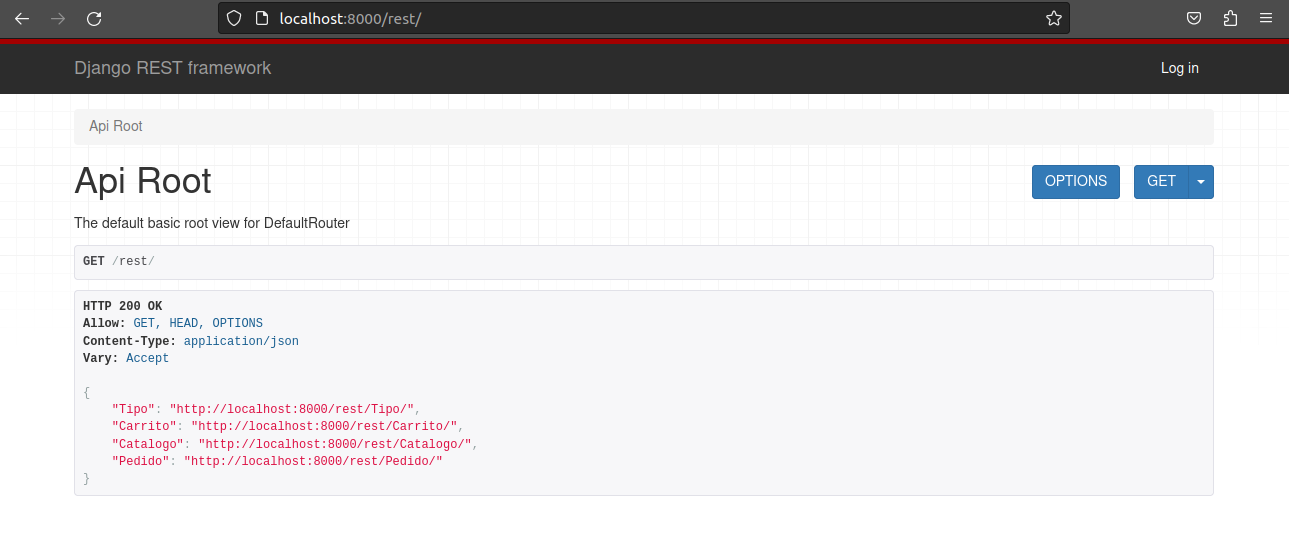
\includegraphics[scale=0.4,keepaspectratio]{img/Captura desde 2023-07-21 08-23-44.png}
		          %\includesvg{img/automata.svg}
		          %\label{img:mot2}
		          %\caption{Product backlog.}
	            \end{figure}
    \begin{itemize}
        \item En este caso se observa la pagina del framework
    \end{itemize}
        \begin{figure}[H]
		          \centering
		          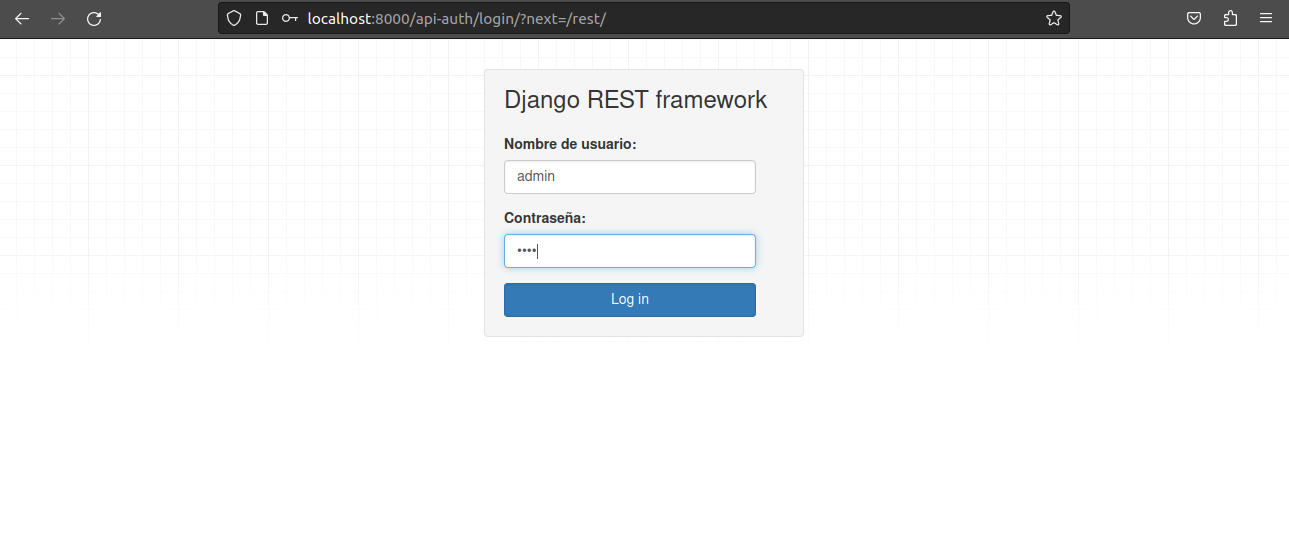
\includegraphics[scale=0.4,keepaspectratio]{img/Captura desde 2023-07-21 08-24-00.png}
		          %\includesvg{img/automata.svg}
		          %\label{img:mot2}
		          %\caption{Product backlog.}
	            \end{figure}
    \begin{itemize}
        \item Vista del login
    \end{itemize}
            \begin{figure}[H]
		          \centering
		          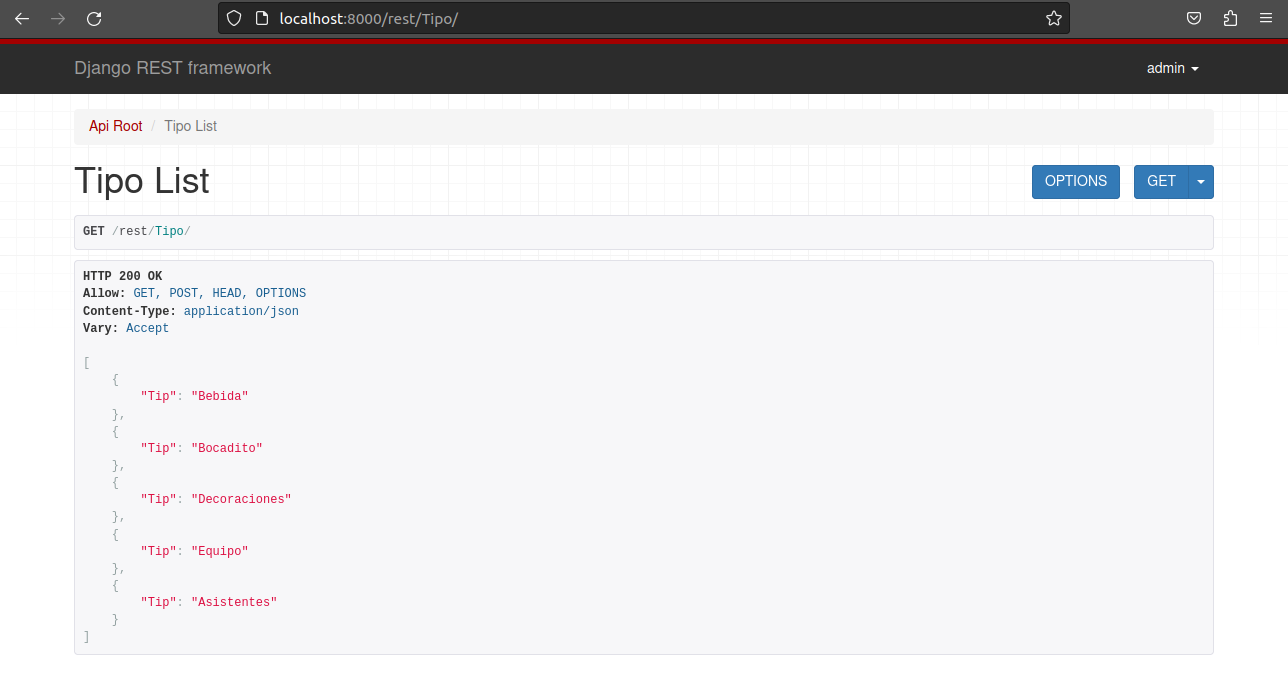
\includegraphics[scale=0.4,keepaspectratio]{img/Captura desde 2023-07-21 08-24-17.png}
		          %\includesvg{img/automata.svg}
		          %\label{img:mot2}
		          %\caption{Product backlog.}
	            \end{figure}
    \begin{itemize}
        \item Vista del model Tipo
    \end{itemize}
    \begin{figure}[H]
		          \centering
		          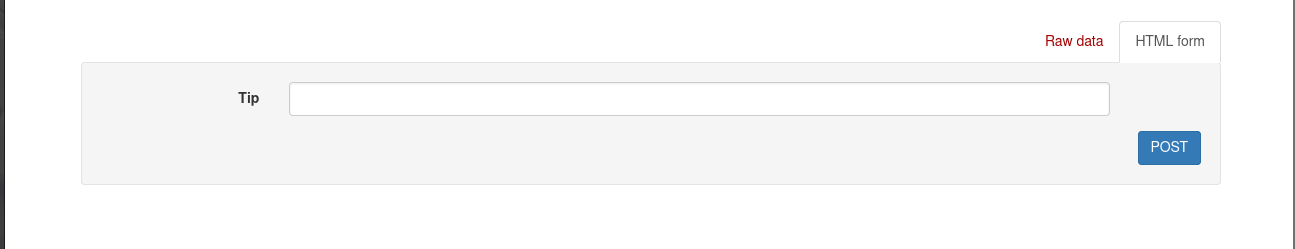
\includegraphics[scale=0.4,keepaspectratio]{img/Captura desde 2023-07-21 08-24-28.png}
		          %\includesvg{img/automata.svg}
		          %\label{img:mot2}
		          %\caption{Product backlog.}
	            \end{figure}
    \begin{itemize}
        \item Vista del PUT
    \end{itemize}
        \begin{figure}[H]
		          \centering
		          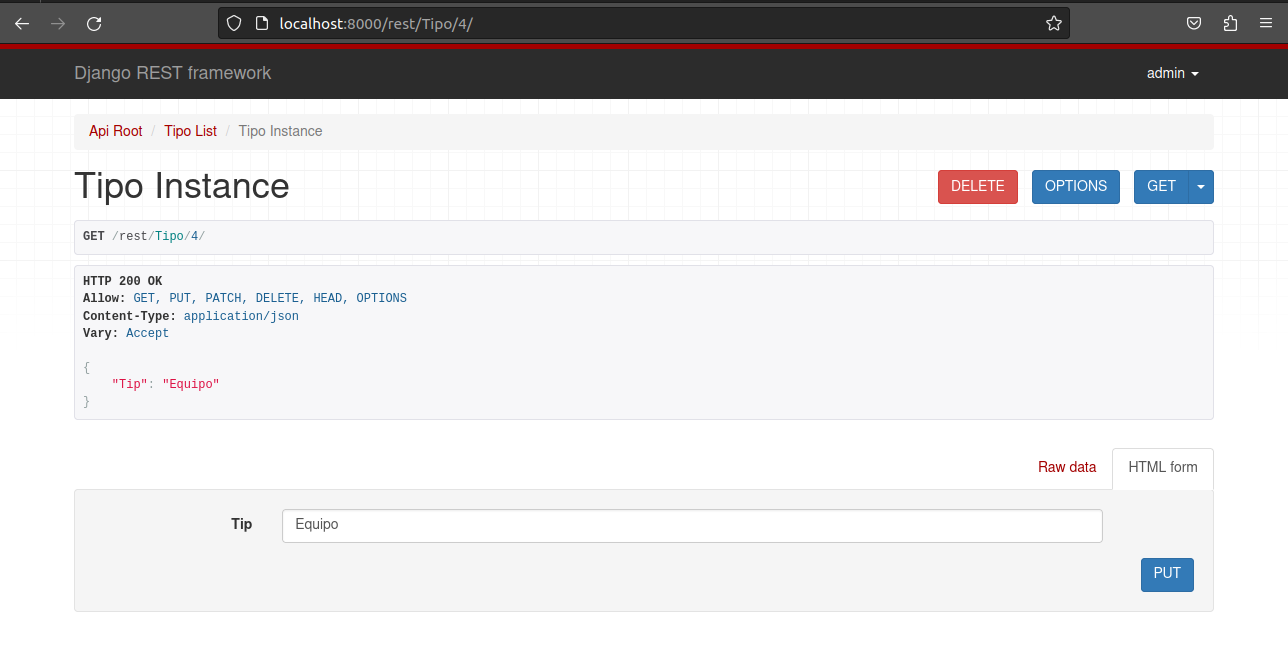
\includegraphics[scale=0.4,keepaspectratio]{img/Captura desde 2023-07-21 08-24-51.png}
		          %\includesvg{img/automata.svg}
		          %\label{img:mot2}
		          %\caption{Product backlog.}
	            \end{figure}
    \begin{itemize}
        \item Vista del Delete, Put, Get; de un objeto.
    \end{itemize}
    \subsection{Commit-GITUHUB}
    \begin{figure}[H]
		          \centering
		          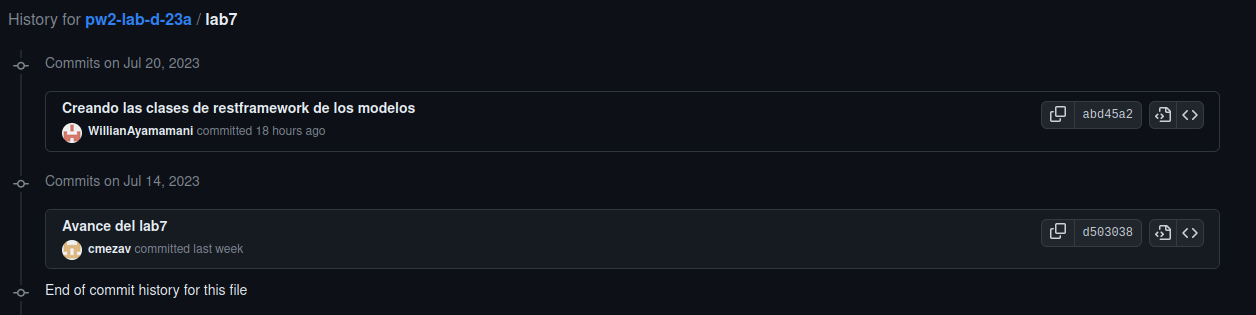
\includegraphics[scale=0.4,keepaspectratio]{img/Captura desde 2023-07-21 09-02-32.png}
		          %\includesvg{img/automata.svg}
		          %\label{img:mot2}
		          %\caption{Product backlog.}
	\end{figure}
    \subsection{USUARIO}
        \begin{lstlisting}[language=bash,caption={Credenciales}][H]
    		          USUARIO:
                        name:Lucho
                        password:1234
                    ADMIN:
                        name:admin
                        password:1234
    	\end{lstlisting}
	\subsection{Estructura de laboratorio 07}
	\begin{itemize}	
		\item El contenido que se entrega en este laboratorio es el siguiente:
	\end{itemize}
\begin{lstlisting}[style=ascii-tree]
\end{lstlisting}    


	\section{\textcolor{red}{Rúbricas}}
	
	\subsection{\textcolor{red}{Entregable Informe}}
	\begin{table}[H]
		\caption{Tipo de Informe}
		\setlength{\tabcolsep}{0.5em} % for the horizontal padding
		{\renewcommand{\arraystretch}{1.5}% for the vertical padding
		\begin{tabular}{|p{3cm}|p{12cm}|}
			\hline
			\multicolumn{2}{|c|}{\textbf{\textcolor{red}{Informe}}}  \\
			\hline 
			\textbf{\textcolor{red}{Latex}} & \textcolor{blue}{El informe está en formato PDF desde Latex,  con un formato limpio (buena presentación) y facil de leer.}   \\ 
			\hline 
			
			
		\end{tabular}
	}
	\end{table}
	
	\clearpage
	
	\subsection{\textcolor{red}{Rúbrica para el contenido del Informe y demostración}}
	\begin{itemize}			
		\item El alumno debe marcar o dejar en blanco en celdas de la columna \textbf{Checklist} si cumplio con el ítem correspondiente.
		\item Si un alumno supera la fecha de entrega,  su calificación será sobre la nota mínima aprobada, siempre y cuando cumpla con todos lo items.
		\item El alumno debe autocalificarse en la columna \textbf{Estudiante} de acuerdo a la siguiente tabla:
	
		\begin{table}[ht]
			\caption{Niveles de desempeño}
			\begin{center}
			\begin{tabular}{ccccc}
    			\hline
    			 & \multicolumn{4}{c}{Nivel}\\
    			\cline{1-5}
    			\textbf{Puntos} & Insatisfactorio 25\%& En Proceso 50\% & Satisfactorio 75\% & Sobresaliente 100\%\\
    			\textbf{2.0}&0.5&1.0&1.5&2.0\\
    			\textbf{4.0}&1.0&2.0&3.0&4.0\\
    		\hline
			\end{tabular}
		\end{center}
	\end{table}	
	
	\end{itemize}
	
	\begin{table}[H]
		\caption{Rúbrica para contenido del Informe y demostración}
		\setlength{\tabcolsep}{0.5em} % for the horizontal padding
		{\renewcommand{\arraystretch}{1.5}% for the vertical padding
		%\begin{center}
		\begin{tabular}{|p{2.7cm}|p{7cm}|x{1.3cm}|p{1.2cm}|p{1.5cm}|p{1.1cm}|}
			\hline
    		\multicolumn{2}{|c|}{Contenido y demostración} & Puntos & Checklist & Estudiante & Profesor\\
			\hline
			\textbf{1. GitHub} & Hay enlace URL activo del directorio para el  laboratorio hacia su repositorio GitHub con código fuente terminado y fácil de revisar. &2 &X &2 & \\ 
			\hline
			\textbf{2. Commits} &  Hay capturas de pantalla de los commits más importantes con sus explicaciones detalladas. (El profesor puede preguntar para refrendar calificación). &4 &X &2 & \\ 
			\hline 
			\textbf{3. Código fuente} &  Hay porciones de código fuente importantes con numeración y explicaciones detalladas de sus funciones. &2 &X &1 & \\ 
			\hline 
			\textbf{4. Ejecución} & Se incluyen ejecuciones/pruebas del código fuente  explicadas gradualmente. &2 &X &1 & \\ 
			\hline			
			\textbf{5. Pregunta} & Se responde con completitud a la pregunta formulada en la tarea.  (El profesor puede preguntar para refrendar calificación).  &2 &X &2 & \\ 
			\hline	
			\textbf{6. Fechas} & Las fechas de modificación del código fuente estan dentro de los plazos de fecha de entrega establecidos. &2 &X &1 & \\ 
			\hline 
			\textbf{7. Ortografía} & El documento no muestra errores ortográficos. &2 &X &2 & \\ 
			\hline 
			\textbf{8. Madurez} & El Informe muestra de manera general una evolución de la madurez del código fuente,  explicaciones puntuales pero precisas y un acabado impecable.   (El profesor puede preguntar para refrendar calificación).  &4 &X &1 & \\ 
			\hline
			\multicolumn{2}{|c|}{\textbf{Total}} &20 & &12 & \\ 
			\hline
		\end{tabular}
		%\end{center}
		%\label{tab:multicol}
		}
	\end{table}
	
\clearpage

\section{Referencias}
\begin{itemize}			
    \item \url{https://github.com/WillianAyamamani/pw2-lab-d-23a/tree/main/lab7}
\end{itemize}	
	
%\clearpage
%\bibliographystyle{apalike}
%\bibliographystyle{IEEEtranN}
%\bibliography{bibliography}
			
\end{document}